\documentclass[hyperref={pdfpagelabels=false},usepdftitle=false]{beamer}
\usepackage{../templates/myStyle}
\setbeamertemplate{caption}{\raggedright\insertcaption\par}
\begin{document}

\title{\titleText}
\subtitle{}
\author{\tutor}
\date{17. Februar 2016}
\subject{Seminar Informatik}

\frame{\titlepage}

%\frame{
%    \frametitle{Inhalte}
%    \setcounter{tocdepth}{1}
%    \tableofcontents
%    \setcounter{tocdepth}{2}
%}

%!TEX root = Presentation-Thoma.tex

\section{Szenario}
\subsection{Semantische Segmentierung}
\begin{frame}{Semantische Segmentierung}
    \begin{figure}[ht]
        \begin{minipage}[b]{0.45\linewidth}
            \centering
            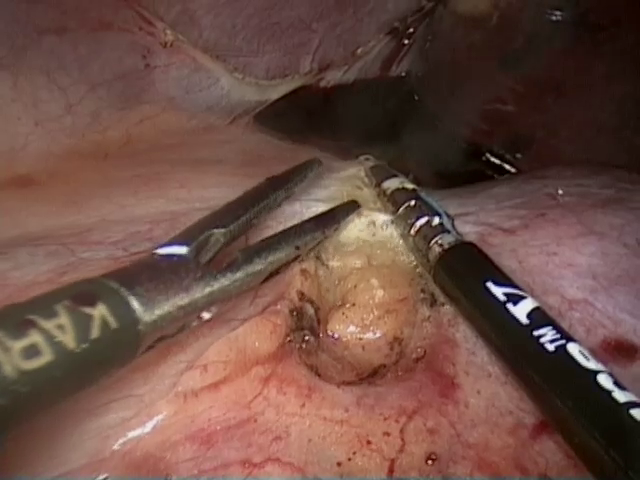
\includegraphics[width=\textwidth]{../images/img_35_raw.png}
            \caption{[Maier-Hein et al, 2014]\hspace{\textwidth}Input}
            \label{fig:input}
        \end{minipage}
        \hspace{0.5cm}
        \begin{minipage}[b]{0.45\linewidth}
            \centering
            
\includegraphics[width=\textwidth]{../images/img_35_label.png}
            \caption{[Maier-Hein et al, 2014]\hspace{\textwidth}Label / Output}
            \label{fig:label}
        \end{minipage}
    \end{figure}
\end{frame}

\begin{frame}{Semantische Segmentierung}
    \begin{figure}[ht]
        \begin{minipage}[b]{0.45\linewidth}
            \centering
            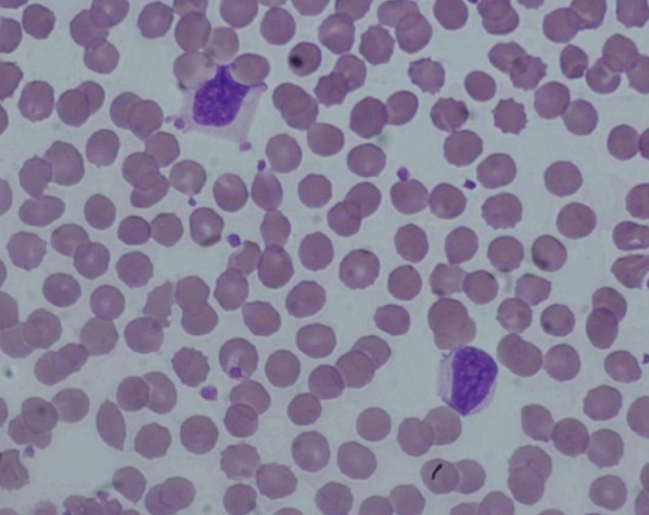
\includegraphics[width=\textwidth]{../images/red-blood.png}
            \caption{[Sharif 2012] Rote Blutkörperchen}
            \label{fig:red-blood}
        \end{minipage}
        \hspace{0.5cm}
        \begin{minipage}[b]{0.45\linewidth}
            \centering
            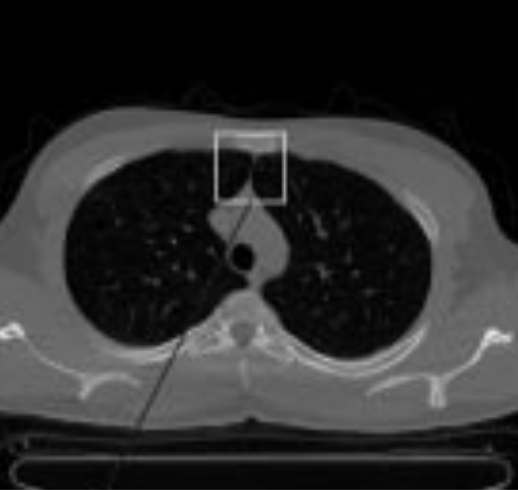
\includegraphics[width=\textwidth]{../images/lung.png}
            \caption{[Hu 2001] Lunge}
            \label{fig:lung}
        \end{minipage}
    \end{figure}
\end{frame}

\begin{frame}{Semantische Segmentierung}
    \begin{figure}[ht]
        \begin{minipage}[b]{0.45\linewidth}
            \centering
            
\includegraphics[width=\textwidth]{../images/mammography.png}
            \caption{[Pham 2000] Mammographie}
            \label{fig:mammographie}
        \end{minipage}
        \hspace{0.5cm}
        \begin{minipage}[b]{0.45\linewidth}
            \centering
            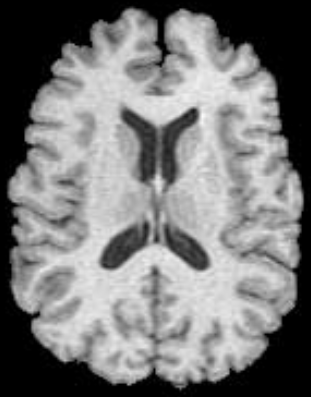
\includegraphics[width=\textwidth]{../images/brain-mr.png}
            \caption{[Pham 2000] Gehirn}
            \label{fig:lung}
        \end{minipage}
    \end{figure}
\end{frame}

%\framedgraphic{Semantische Segmentierung}{../images/sematic-segmentation-fields.jpg}

%!TEX root = Presentation-Thoma.tex
\section{Taxonomie}
\subsection{Taxonomie}

\begin{frame}{Taxonomie}
    \begin{enumerate}
        \item Klassen
        \item Pixelzugehörigkeit
        \item Daten
        \item Betriebsart
    \end{enumerate}
\end{frame}

\begin{frame}{Taxonomie: Klassen}
    \begin{enumerate}
        \item Welche Klassen gibt es?
        \item Gibt es eine \textbf{void} Klasse?
    \end{enumerate}
\end{frame}

\begin{frame}{Taxonomie: Pixelzugehörigkeit}
    \begin{center}
        Zu wie vielen Klassen kann ein Pixel gehören?\\

        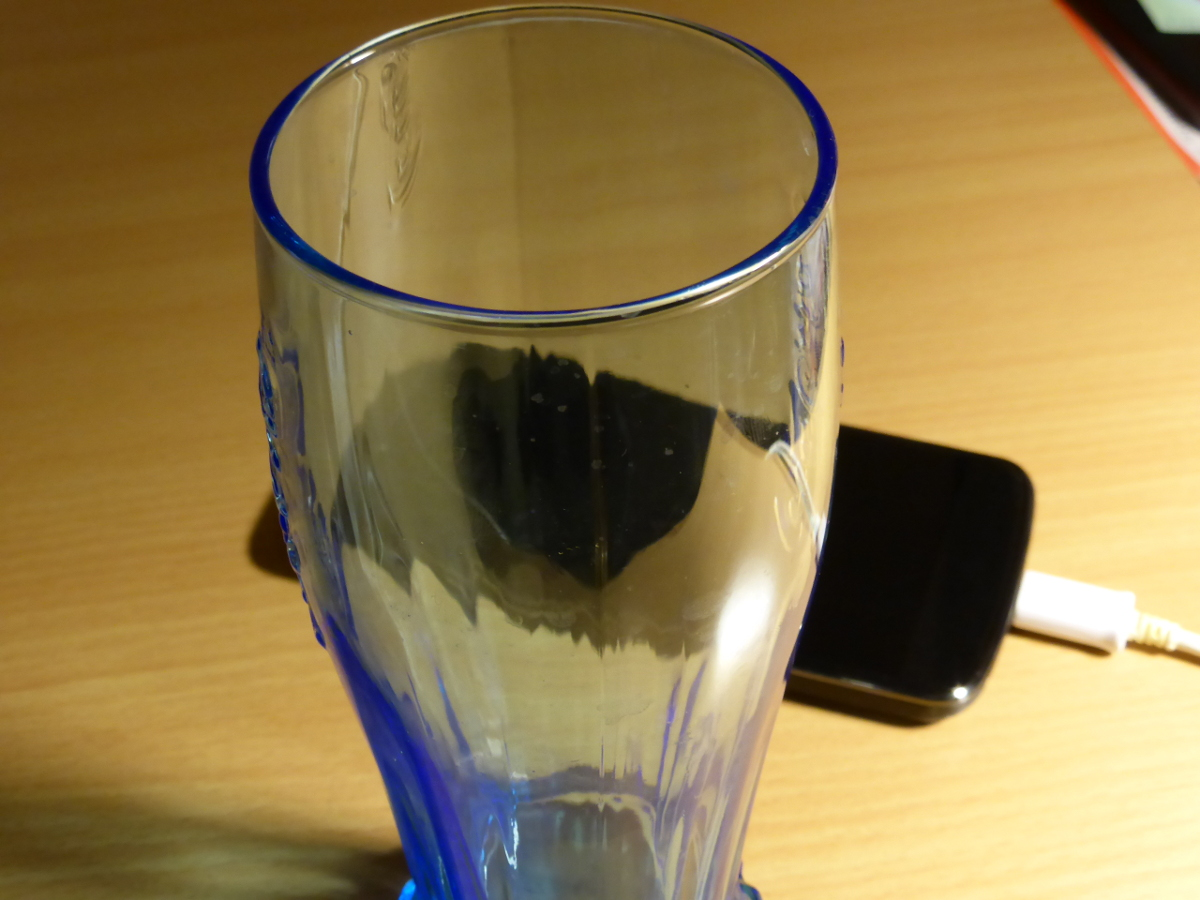
\includegraphics[width=0.6\textwidth]{../images/glass-smartphone-table-2.jpg}
    \end{center}
\end{frame}

\begin{frame}{Taxonomie: Daten}
    \begin{itemize}
        \item Grau oder Farbig?
        \item Tiefeninformation?
        \item Einzelbilder, Stero-Bilder oder Co-Segmentierung?
        \item 2D oder 3D?
    \end{itemize}
\end{frame}

\begin{frame}{Taxonomie: Betriebsart}
    \begin{itemize}
        \item aktiv
        \item passiv
        \begin{itemize}
            \item interaktiv
            \item vollautomatisch
        \end{itemize}
    \end{itemize}
    \begin{figure}[ht]
            \centering
            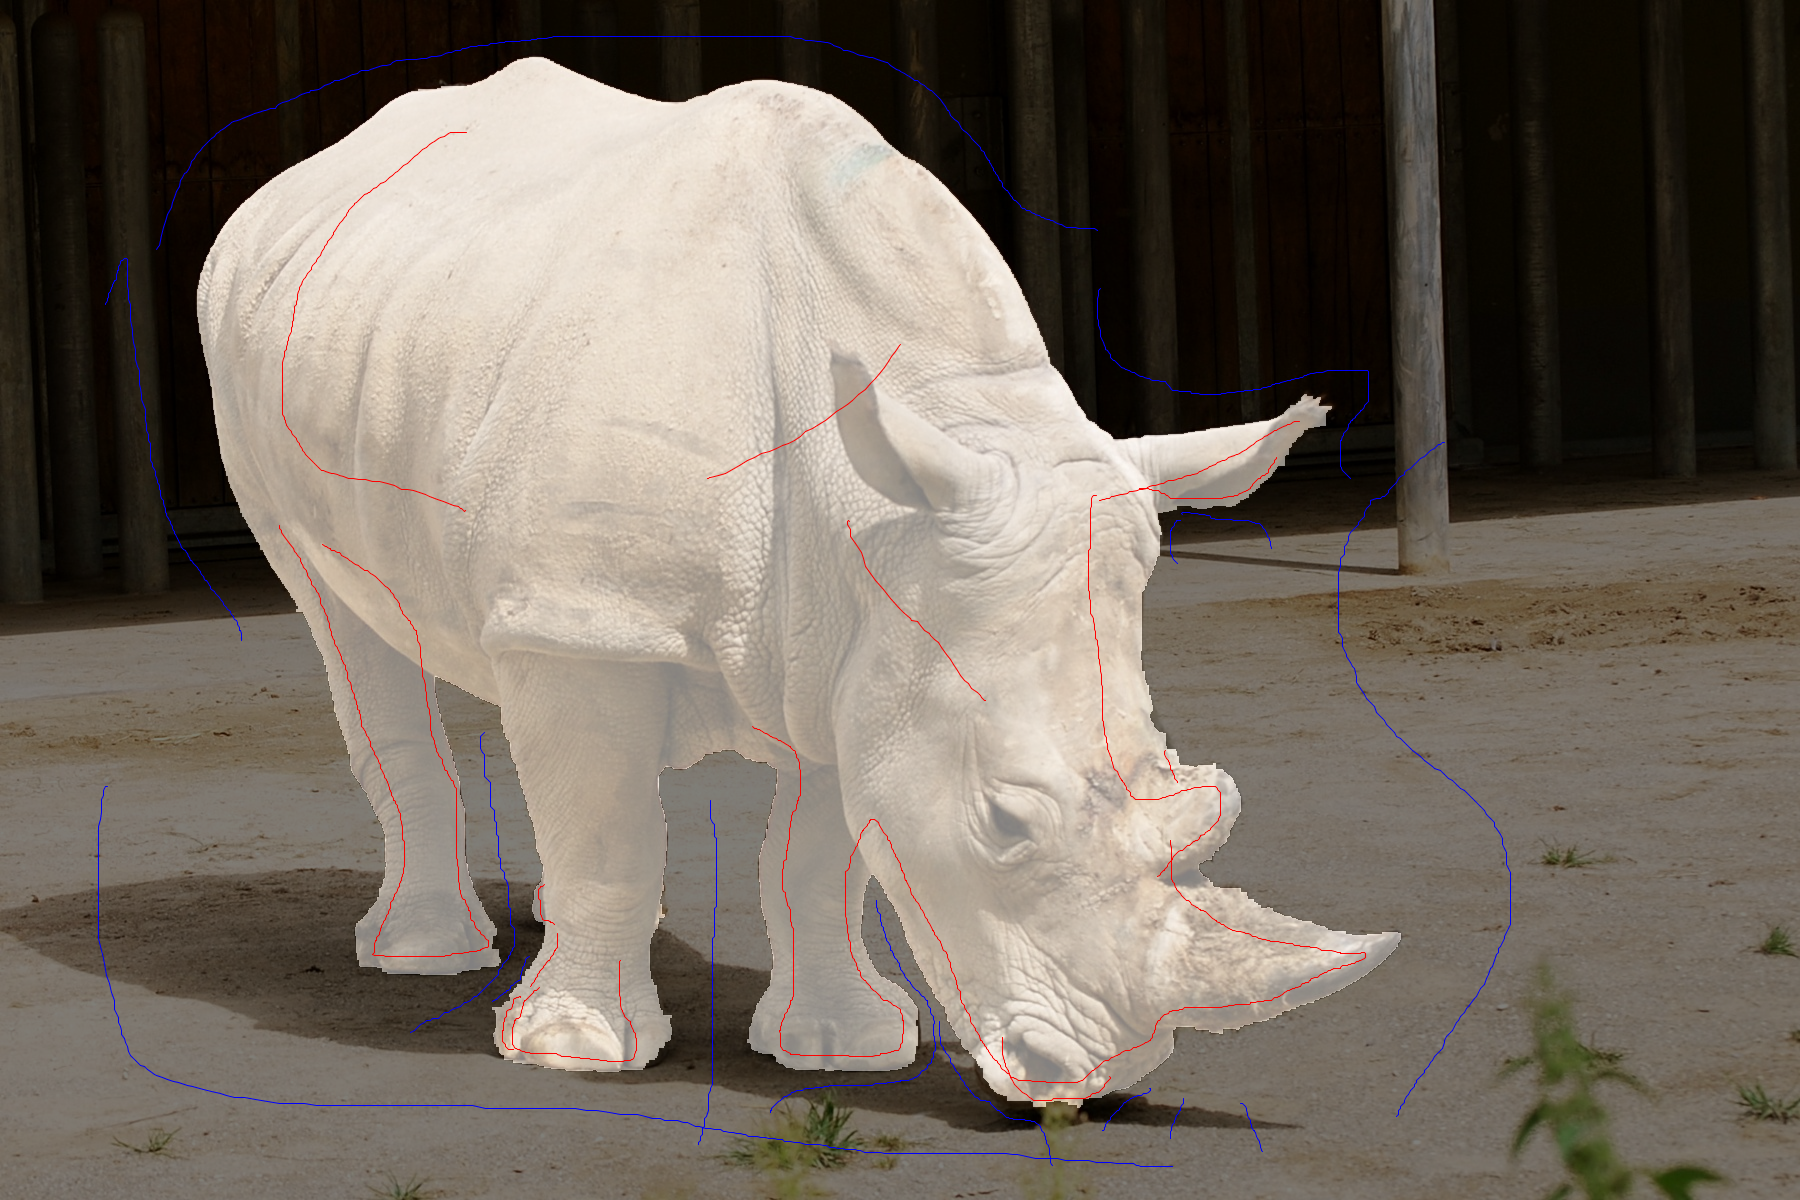
\includegraphics[width=0.45\textwidth]{../images/TIP-1.jpg}
            \caption{Interaktive Segmentierung}
    \end{figure}
    {\tiny Bildquelle: \href{http://staff.ustc.edu.cn/~juyong/publications.html}{staff.ustc.edu.cn/~juyong/publications.html}}
\end{frame}

\begin{frame}{Hier:}
    \begin{itemize}
        \item Klassen: Beliebig, aber meist ohne \texttt{void}.
        \item Pixelzugehörigkeit: Genau eine Klasse pro Pixel.
        \item Daten:
        \begin{itemize}
            \item grau oder farbig
            \item keine Tiefeninformationen
            \item Einzelbilder
            \item 2D
        \end{itemize}
        \item Betriebsmodus:
        \begin{itemize}
            \item passiv, vollautomatisch
        \end{itemize}
    \end{itemize}
\end{frame}

%!TEX root = Presentation-Thoma.tex
\section{Verfahren}
\subsection{Verfahren}

\begin{frame}{Verfahren}
    Allgemein
    \begin{itemize}
        \item \textbf{Sliding Window + Allgemeiner Klassifizierer}
        \item Markov Random Field / Conditional Random Field
        \item CNN + Tricks (vgl. Marvin)
    \end{itemize}

    Allgemeine Klassifizierer
    \begin{itemize}
        \item Random Forests
        \item SVMs
        \item Neuronale Netze
    \end{itemize}
\end{frame}

%!TEX root = Presentation-Thoma.tex
\section{Ende}
\subsection{Danke!}
\begin{frame}{Danke!}
    \begin{center}
        \Huge
	    Gibt es Fragen?
    \end{center}
\end{frame}

\subsection{Bildquellen}
\begin{frame}{Bildquellen}
\begin{itemize}
	\item J. M. Sharif, M. F. Miswan, M. A. Ngadi, Md Sah Hj Salam.
          \textit{Red Blood Cell Segmentation Using Masking and Watershed Algorithm: A Preliminary Study}. 2012.
    \item S. Hu, E. Hoffman, J. Reinhardt. \textit{Automatic lung segmentation for accurate quantitation of volumetric X-ray CT images}. 2001.
\end{itemize}
\end{frame}

\subsection{Literatur}
\begin{frame}{Literatur}
\begin{itemize}
    \item J. Shotton, J. Winn, C. Rother and  A. Criminisi: \textit{Textonboost: Joint appearance, shape and context modeling for multi-class object recognition and segmentation}. 2006.
    \item J. Shotton, M. Johnson and R. Cipolla: \textit{Semantic texton forests for image categorization and segmentation}. 2008.
    \item Y. Yang, S. Hallman, D. Ramanan and C. Fowlkes: \textit{Layered object models for image segmentation}. 2012.
    \item Insgesamt 119 Quellen, vgl. Paper für den Rest.
\end{itemize}
\end{frame}

\subsection{Folien, \LaTeX und Material}
\begin{frame}{Folien, \LaTeX und Material}
Der Foliensatz sowie die \LaTeX und Ti\textit{k}Z-Quellen sind unter

\href{https://github.com/MartinThoma/seminar-pixel-exact-classification}{github.com/MartinThoma/seminar-pixel-exact-classification}
\\

Kurz-URL:
\href{http://tinyurl.com/semantic-segmentation}{tinyurl.com/semantic-segmentation}
\end{frame}


\end{document}
